\documentclass[letterpaper]{aamas2009}
%\usepackage{ijcai09}
\usepackage{amssymb}
%\usepackage[english]{babel}
\usepackage{latexsym}
\usepackage{amsfonts}
\usepackage{amsmath}
\usepackage{graphicx}
\usepackage{algorithmic}
\usepackage{times}
\usepackage{subfigure}
%\usepackage{natbib}
%
\def\sharedaffiliation{%
\end{tabular}
\begin{tabular}{c}}
%

\numberofauthors{3} 

\author{\alignauthor Zinovi Rabinovich\\
  \affaddr{Electronics and Computer Science}\\
  \affaddr{University of Southampton}\\
  \affaddr{Southampton, United Kingdom}\\
  \email{zr@ecs.soton.ac.uk}
\alignauthor Lachlan Dufton\\ 
  \affaddr{Cheriton School of Computer Science}\\
  \affaddr{University of Waterloo}\\
  \affaddr{Waterloo, Canada}\\
  \email{ltdufton@cs.uwaterloo.ca}
\alignauthor Kate Larson\\
  \affaddr{Cheriton School of Computer Science}\\
  \affaddr{University of Waterloo}\\
  \affaddr{Waterloo, Canada}\\
  \email{klarson@cs.uwaterloo.ca}
} 

\title{Policy  Teaching by a Modulation of the Transition Model}

\begin{document}

\maketitle

\section{Introduction}
\nocite{taylor_PhD_2008}
\nocite{taylor_stone_2009}
\nocite{fleming_hernandez-hernandez_CDC_97}
\nocite{todorov_2009_framework_sup}
\nocite{todorov_2009_framework}
\nocite{ng_russell_2000}
\nocite{zhang_parkes_2008}
\nocite{zhang_parkes_2009_ed}
\nocite{dufton_larson_2009}
\nocite{banerjee_peng_2005}

Recently, Zhang \emph{et al} introduced a general framework for \emph{environment design}~\cite{Zhang09:General}. In environment design an interested party attempts to influence the behavior of an agent by making limited changes to the agent's environment.  While our model is a particular example of environment design, we note that our instantiation differs significantly from the particular cases studied by Zhang \emph{et al}.  
In particular, Zhang \emph{et al} have allowed their interested party to modify the cost function of an agent in a linear programming example~\cite{Zhang09:General}, or to modify the rewards of an agent acting in an environment modeled as an MDP~\cite{zhang_parkes_2008,Zhang09:Policy}.
We, however, study the implications of allowing the interested party (teacher, in our model) to modify the \emph{dynamics} of the environment, while leaving the reward function of the agent alone.  


%Zhang et al~\cite{Zhang09:Policy}  looked at environment design (include citation for aaai 2008 
%paper).  Had an interested party that tries to influence an agent's behavior by making limited 
%changes to the agent's environment. Thus our work fits into this paradigm.  

%The difference is that they were interested in influencing the agent's reward function, by providing 
%positive incentives $\Delta:S\mapsto \mathbb{R}$, and then allowing the agent to re-act to the 
%change in reward function.  Additionally the placement of incentives  is only through the reward 
%function.  That is, their policy-teaching process had the interested party modifying the agent's 
%reward function tp affect it's policy.

%%Zhang et al have investigated this model as it applies to value-based policy  teaching~
%%\cite{zhang_parkes_2008}. In this work they studied how the interested party 
%could induce a policy 
%%that maximized \emph{it's} value, when using limited incentives.  
%In follow-up work, Zhang et al~
%%\cite{Zhang09:Policy}  studied the policy-teaching setup where the goal is to teach 
%a pre-specified 
%%desired policy.  This is what we are doing, but we are going to go about it in a different way -- 
%%though modifications to the dynamics of the underlying MDP.

%%Zhang et al~\cite{Zhang09:General} introduce a general framework for environment design.
% Our model does fit into their definition. However, our particular instantiation 
%%has not been looked at. 
%%Also their focus is different. In particular, it looks as though what we are interested 
%in is actualy an instance of their "static formulation" since the "dynamic formulation" really
% focuses on eliciting model parameters.  While we do repeatedly interact with the agent 
% in our model, we do start with the assumption that the interested party does know the model.
%%Their particular instantiation involves a linear programming example where the
% interested party can modify the costs incurred by the agent.
%%I need to go back and re-read the paper - part of it is so general to be not
% particularly useful, while the other part is so specific to not be particularly useful.

%%%%%%%%%%%%%%%%%%%%%%%%%%%%%%
\section{Interaction Model}\label{sec: GeneralModel}
%%%%%%%%%%%%%%%%%%%%%%%%%%%%%%

In this section we provide a high level description of the problem and general framework.
In the next section we provide a particular instantiation of our framework.

Our framework consists of a stochastic environment and two agents, a \emph{learner} and a 
\emph{teacher}.   The learner acts within the environment, taking actions and receiving feedback in 
the form of rewards, which depend on the action taken and the current state of the environment in 
which the agent finds itself.  We assume that the learner is rational and thus attempts to find a 
\emph{policy} which describes what action to take in each environment state,  that maximises its 
expected reward.  The teacher, on the other hand, does not act \emph{in} the environment, but rather acts \emph{on} the environment.  In particular, the teacher has some desired \emph{reference policy}, $\pi^*$, that it wishes the learner to follow, but is unable to force the agent to take any particular action.  Instead, it is able to modify the environment's \emph{dynamics} in order to  influence the policy choice of the learner. That is, the teacher's actions are able to influence the way the environment state changes in response to the learner's actions, and thus influence the policy of the learner. Dynamics modifications come at a cost, however, and thus the goal of the teacher is to minimize the modifications it must make to the environment dynamics while at the same time ensuring that the policy followed by the learner is close enough to the desired reference policy.




%Our interaction framework consists of a dynamic stochastic environment
%that is influenced by two agents, a {\em learner} and a {\em
%  teacher}. The learner agent receives a direct feedback from the
%environment in form of a reward, that depends on the change in the
%environment's state and the action chosen by the learner. We assume
%that the learner is rational and, therefore, seeks an action policy
%that will maximise its expected reward. To achieve this goal the
%learner employs a publicly known iterative computation or a learning
%algorithm, depending on environment model availability. At each
%iteration of the algorithm, the chosen policy is compared with some
%ideal or {\em reference} policy held by the teacher agent. The
%difference between the two policies determines the cost of that stage
%for the teacher agent. The teacher agent may attempt to influence the
%learner's policy calculation by modifying the environment
%dynamics. That is, the teacher's actions influence the way the
%environment state changes in response to the learner's
%actions. However, such modulation incurs additional cost to the
%teacher agent. Further away the teacher pushes the environment from a
%certain nominal or {\em passive} dynamics, higher the cost. In this
%interaction framework, we would be interested to find a sequence of
%teacher's actions that optimally balances the two costs: distance of
%the learner's policy from the reference and the cost of the
%environment modification.

We model the problem by $\langle S, A, c,\gamma, U,T\rangle$ where:
%
%To instantiate the above framework, we will consider for the remainder
%of this paper the following Markovian environment tuple $<S,A,U,T,R>$,
%where:
\begin{itemize}
\item $S$ is the set of states, 
\item $A$ is the set of actions available to the learner,
\item  $c:S\times A\times S\rightarrow\mathbf{R}$ is the reward (or
  cost) function of the learner. $c(s',a,s)$ is the reward received by
  the learner if it has applied action $a\in A$ and the environment
  moved from state $s\in S$ to state $s'\in S$,
\item $\gamma \in (0,1)$ is a discount factor,   

\item $U$ is the set of actions (modifications to the environment)  that the teacher can apply and $u_t\in U$ is the modification made at time $t$, 

\item $T:S\times A\times U\rightarrow\Delta(S)$ describes the environment dynamics where 
$T_u(s'|s,a)\equiv T(s'|s,a,u)$ is the probability that the state will change from $s$ to $s'$ if the learner has
  applied action $a\in A$ and the teacher chose  environment
  modification $u\in U$.

%Denote $T_{u_t}(s'|s,a)=T(s'|s,a,u_t)$. 
 
 %% KATE NEEDS TO THINK ABOUT THE NEXT BIT SINCE SHE DOES NOT LIKE THE 
 %% NOTATION.
We assume that there exist a null
  modification $u^*\in U$, so that $T^*=T_{u^*}$ are the nominal,
  passive dynamics of the environment.
\end{itemize}

While applying its iterative policy calculation algorithm, the learner
faces a sequence of Markov Decision Problems (MDPs)~\cite{puterman_book_94}
$<S,A,U,T_{u_t},R>$, although it is not aware of the dynamics
modulation and proceeds as if they were homogeneous. That is, at every
stage the learner seeks an action policy of the form
$\pi:S\rightarrow\Delta(A)$ that would produce the highest expected
reward if $T_{u_t}$ would persist indefinitely.\footnote{This latter
  assumption is explicit only if the learner actually has access to
  the environment model. For most standard RL algorithms this
  assumption would hold implicitly.}

Now, denote $x_t$ the internal state of the learner's policy
computation at iteration $t$, and let
$\pi_t=\pi(x_t):S\rightarrow\Delta(A)$ be the policy that corresponds
to that computation state. Also, denote $\pi^*$ the ideal reference
action policy of the learner. Then at time $t$ the teacher incurs cost
$Cost(\pi_t,u_t)$ that combines the distance between $\pi_t$ and
$\pi^*$ and between $T_{u_t}$ and $T^*$. The overall optimisation
problem for the teacher is as follows, where $x_t=F(x_{t-1},u_t)$
denotes one step of the learner's computation algorithm and $x_0$ is
known:
\begin{eqnarray*}
&\min\limits_{u_t}\sum\limits_{t=1}^{t_{max}}Cost(\pi_t,u_t)\\
&s.t.\\
&\pi_t=\pi(x_t)\\
&x_t=F(x_{t-1},u_t)
\end{eqnarray*}

Notice that the above formulation is generic with respect to the
actual algorithm employed by the learner agent. The formalism captures
both policy and value iteration algorithms, both with given and
learned environment model. It even captures the case where the learner
is capable of transfer learning. In this case learner's state $x_t$
will include structural knowledge gathered thus far from the
interaction with the environment. 

The teacher-learner interaction framework, as we have describe it
above, can also adopt various cost functions that describe how the
teacher fuses the environment modification effort and the distance of
the learner from the reference policy. However, in this work we adopt
a specific cost function based on the Kullback-Leibler divergence
rate. This enables an autonomic balancing between the two costs. It also
has the additional benefit to concentrate the cost dependency on those
portions of the environment dynamics that are most relevant to the
current action policy choice by the learner. In the following
subsection we describe our teacher's cost function in more detail.

\subsection{Teacher's Cost Computation}
As a measure of cost we will use Kullback-Leibler divergence rate
between two processes formed by the application of the teacher's
augmentation $u_t$ and the learner's policy $\pi_t$. More specifically,
consider the stochastic process over the state-action pairs formed by
the application of the learner's policy in the modified environment at
time $t$: \\
\centerline{$
P_t(s',a'|s,a)=T_{u_t}(s'|s,a)\pi_t(a'|s')
$}

Similarly, denote $P^*(s',a'|s,a)=T^*(s'|s,a)\pi^*(a'|s')$.

The process $P_t$ has a stationary distribution $q_t$ over $S\times
A$, so that $q_t=P_tq_t$. Notably, the stationary distribution can be
decomposed (with a slight abuse of notation) $q_t(s,a)=q_t(a|s)q_t(s)$
and then expressed by the following equations:
%% \begin{eqnarray*}
%% q_t&=&q_t(a'|s')q_t(s')=P_tq_t\\
%% &=&\sum\limits_{s,a}T_{u_t}(s'|s,a)\pi_t(a'|s')q_t(a|s)q_t(s)\\
%% &=&\pi_t(a'|s')\sum\limits_sq_t(s)\sum\limits_aT_{u_t}(s'|s,a)q_t(a|s)\\
%% &&\{\displaystyle{substitute}\ \ q_t(\cdot|\cdot)\Leftarrow\pi_t(\cdot|\cdot)\}\\
%% &=&\pi_t(a'|s')\sum\limits_sq_t(s)\sum\limits_aT_{u_t}(s'|s,a)\pi_t(a|s)\\
%% &&\{\displaystyle{denote}\ \ \Tilde{T}_{u_t}(s'|s)=\sum\limits_aT_{u_t}(s'|s,a)\pi_t(a|s)\}\\
%% &=&\pi_t(a'|s')\sum\limits_sq_t(s)\Tilde{T}_{u_t}(s'|s)
%% \end{eqnarray*}
%% so that
\begin{eqnarray*}
q_t(s',a')&=&\pi_t(a'|s')q_t(s')\ \ \displaystyle{where}\\
q_t(s')&=&\sum\limits_s\Tilde{T}_{u_t}(s'|s)q_t(s)
\end{eqnarray*}

Assuming that $P_t$ and $P^*$ are irreducible w.r.t. $S\times A$ the
Kullback-Leibler divergence rate, $KLR$, can be computed~\cite{rached_alajaji_campbell_2004} to form the
necessary cost function as follows:
$$
Cost(u_t,\pi_t)=KLR(P_t\|P^*)=\sum\limits_{s,a}q_t(s,a)D^{KL}_t(s,a),$$
where $$D^{KL}_t(s,a)=\sum\limits_{s',a'}P_t(s',a'|s,a)\log\frac{P_t(s',a'|s,a)}{P^*(s',a'|s,a)},
$$

The overall generic teacher optimisation problem (TOP) is depicted in
Figure~\ref{t_opt}. Notice that this formulation retains complete
flexibility with respect to the specific algorithm selected by the
learner to optimise its policy. However, to provide further intuition
and demonstrate the feasibility of the approach we instantiate the
algorithm $F$ to be the Policy Iteration algorithm.
\begin{figure}[ht]
\begin{tabular}{|c|} \hline \parbox{3.2 in} {\center 
$\arg\min\limits_{u_t}\sum\limits_{t=1}^{t_{max}}\sum\limits_{s,a}\pi_t(a|s)q_t(s)D^{KL}_t(s,a)$\\
s.t.\\
$\pi_t=\pi(x_t)$\\
$x_t=F(x_{t-1},u_t)$\\
$x_0\ \ \displaystyle{is\ \ given}$\\
$D^{KL}_t(s,a)=\sum\limits_{s',a'}T_{u_t}(s'|a,s)\pi_t(a'|s')\log\frac{T_{u_t}(s'|a,s)\pi_t(a'|s')}{T^*(s'|a,s)\pi^*(a'|s')}$\\
$q_t(s')=\sum\limits_s\Tilde{T}_{u_t}(s'|s)q_t(s)$\\
$\Tilde{T}_{u_t}(s'|s)=\sum\limits_aT_{u_t}(s'|s,a)\pi_t(a|s)\}$\\\ \\
}\\ \hline \end{tabular}
\caption{\label{t_opt}The complete generic TOP}
\end{figure}

\subsection{TOP with Policy Iteration}
The policy iteration (PI) algorithm is an iterative computation
algorithm that operates over an explicitly given MDP. Given the policy
of the previous iteration, $\pi_{t-1}$, PI first computes the so
called value function $V_t(s)$ for that policy. $V_t(s)$ represents
the expected total discounted reward that can be achieved if the
environment starts at state $s$ and the agent follows $\pi_{t-1}$. PI
then adopts a different policy for the current stage, one that takes
advantage of the $V_t$ guarantees. Formally instantiating our
learner's state update $F(x_t,u)$ by PI leads to the following set of
equations:
{\center 
$V_t(s)=\sum\limits_{s'}T_{u_t}(s'|s,\pi_{t-1}(s))\left[
c(s',\pi_{t-1}(s),s)+\gamma V_t(s')
\right]$\\
$\pi_t(a|s)=\frac{1}{Z_t(s)}\exp\left(\tau_t\sum\limits_{s'}T_{u_t}(s'|s,a)\left[
c(s',a,s)+\gamma V_t(s')
\right]\right)$\\
$Z_t(s)=\sum\limits_a\exp\left(\tau_t\sum\limits_{s'}T_{u_t}(s'|s,a)\left[
c(s',a,s)+\gamma V_t(s')
\right]\right)$\\
}
The parameter $\tau_t$ denotes a so called temperature scale that
shifts the soft-max towards the greedy maximum selection. Substituting
the above into the standard TOP formulation leads to a TOP-PI
optimisation problem depicted in Figure~\ref{t_opt_PI}.
\begin{figure}[th]
\begin{tabular}{|c|} \hline \parbox{3.2 in} {\center 
$\arg\min\limits_{u_t}\sum\limits_{t=1}^{t_{max}}\sum\limits_{s,a}\pi_t(a|s)q_t(s)D^{KL}_t(s,a)$\\
$s.t.$\\
$V_t(s)=\sum\limits_{s'}T_{u_t}(s'|s,\pi_{t-1}(s))\left[
c(s',\pi_{t-1}(s),s)+\gamma V_t(s')
\right]$\\
$\pi_t(a|s)=\frac{\exp\left(\tau_t\sum\limits_{s'}T_{u_t}(s'|s,a)\left[
c(s',a,s)+\gamma V_t(s')
\right]\right)}{Z_t(s)}$\\
$Z_t(s)=\sum\limits_a\exp\left(\tau_t\sum\limits_{s'}T_{u_t}(s'|s,a)\left[
c(s',a,s)+\gamma V_t(s')
\right]\right)$\\
$\pi_0\ \ \displaystyle{given}$\\
$D^{KL}_t(s,a)=\sum\limits_{s',a'}T_{u_t}(s'|a,s)\pi_t(a'|s')\log\frac{T_{u_t}(s'|a,s)\pi_t(a'|s')}{T^*(s'|a,s)\pi^*(a'|s')}$\\
$q_t(s')=\sum\limits_s\Tilde{T}_{u_t}(s'|s)q_t(s)$\\
$\Tilde{T}_{u_t}(s'|s)=\sum\limits_aT_{u_t}(s'|s,a)\pi_t(a|s)\}$\\\ \\
}\\ \hline \end{tabular}
\caption{\label{t_opt_PI}TOP-PI: The complete and explicit TOP for the
  PI learner}
\end{figure}

\section{Experimental Demonstration}
Consider an learner agent that is tasked with finding an optimal path
for supply transportation between point S and T on a grid. The
learner's reward is initially fixed to be $-1$ for every step it takes
plus some values $R_{ST}$ and $R_{TS}$ for reaching point T from S and
vice versa. In a uniform grid this would be a simple problem, however,
the gird simulates a terrain and cells have an elevation associated
with it. As a result, any movement from one cell to another
neighbouring cell succeeds with a probability proportionate to the
relative elevation of the cells. Consider the situation depicted in Figure~\ref{exp_motion}. 

\begin{figure}[ht]
\centerline{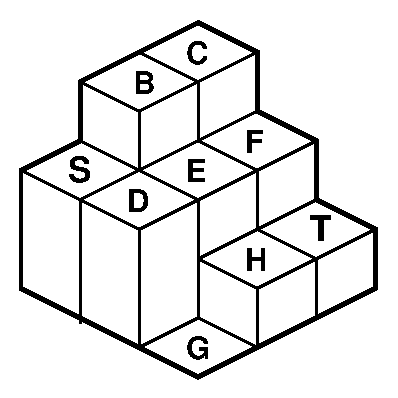
\psfig{file=img/exp_motion.eps,width=5cm}}
\caption{\label{exp_motion}Example of a 3D terrain grid}
\end{figure}

If the cells are of equal elevation, the movement almost always
succeeds, e.g. moving from cell $B$ to cell $C$ in
Figure~\ref{exp_motion}. If the source cell of the motion is lower
than the target cell, then the motion succeeds with low
probability. Furthermore, in this case, a non-zero probability exists
that the direction of motion will be altered. E.g. moving from $H$ to
$E$ is unlikely to succeed, and the agent may end up in $D$, $F$ or
even $G$. If the motion is directed to lower the elevation, it is most
likely will succeed, but also has certain probability to move further
than intended. E.g. moving from $B$ to $E$ is likely to succeed, but
the agent may end up in $H$ or $G$.

Finding an optimal path of motion from $S$ to $T$ and back is,
therefore, becomes non-trivial. Still, if the probabilities of
different transitions are given, the policy iteration algorithm can
easily solve the problem. However, the time it takes the algorithm to
converge to an optimal policy may vary depending on how prominent are
the features of the terrain. Therefore it would be reasonable to
assume that scaling the terrain (and modifying transition
probabilities accordingly) during the initial iterations of learning
will result in faster convergence to the optimal solution. Our
experiments are directed to verify this proposition using our TOP-PI formalism.

{\Large TODO\\ -- CONTINUE WITH REAL DETAILS HERE}

\section{Conclusions and Future Work}

In this paper we have introduced a novel interaction framework between
a teacher and a learner agents. Unlike previous developments in this
area, in our framework the teacher influences the learner indirectly by
modifying the environment away from some normative, passive
dynamics. 

Although in this paper we provide an example based on a learner
executing the policy iteration (PI) algorithm, this limitation is not
a part of our Teacher Optimisation Problem (TOP) framework. Rather it
is a particular instantiation of its principles for the PI
algorithm. As part of our ongoing research we will investigate the
instantiations of TOP with other learning algorithms, particularly
those capable of knowledge transfer.

The cost and the effectiveness of the teaching process in TOP can
be measured simultaneously via the Kullback-Leibler divergence rate
(KLR). Specifically, by measuring the KLR between two state-action
processes engendered by the learner's action policy and the
environment dynamics set by the teacher. The detailed choice of the
two processes depends on the interpretation of this cost. One such
interpretation, as the effort it takes to sustain the teaching process
at any given time, is adopted in this paper. As a result the cost is
the KLR between the current policy-environment combination and the
combination of the reference policy with the passive
dynamics. However, in our future work we intend to explore a different
interpretation -- the total effort invested into the teaching
process. In this case the KLR will be between two consecutive
policy-environment combinations plus some final cost expressed by the
KLR between the final policy-environment pair and the combination of
the reference policy with the passive environment dynamics. 


\bibliographystyle{plain}
\bibliography{teacher_em}

\newpage
\appendix
\section{Intuition}
Given a learner that attempts to find an action policy to optimise its
utility. We can modify the environment response to the learner's
actions and we want to use this capability to enforce learning of a
particular policy of action.

For instance, if a learning agent needs to find an optimal racing path
(see Figure~\ref{race_path}), depending on the terrain it may take long
time to explore all options. By making the terrain features more
prominent at several locations a teacher can facilitate faster
learning of the intended cycle.

\begin{figure*}[ht]
{\center 
\subfigure[Passive dynamics]{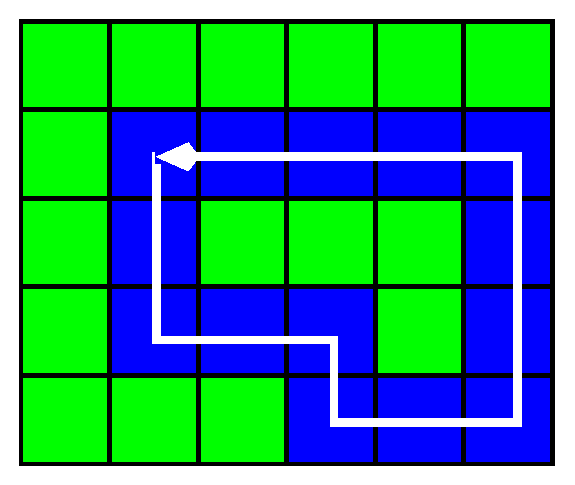
\psfig{file=img/race_track_flat.eps,width=5cm}}
\subfigure[Augmented dynamics]{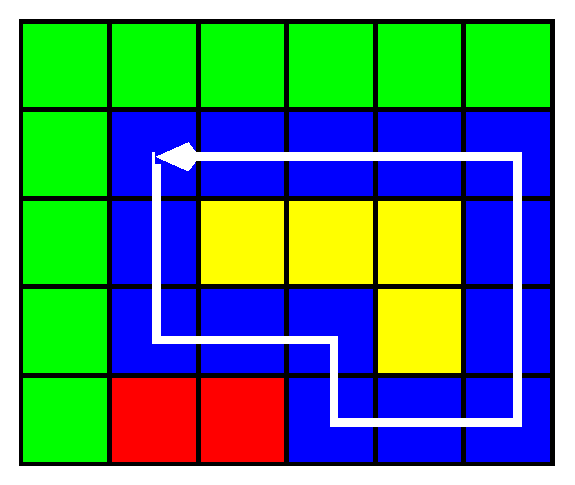
\psfig{file=img/race_track.eps,width=5cm}}\\}
\caption{\label{race_path}Unmodified (passive) and augmented environment dynamics for race path finding (colours naturally encode traversability of the cell)}
\end{figure*}

\end{document}
